\pdfoutput=1
\documentclass[11pt]{article}
\usepackage[T1]{fontenc}
\usepackage[utf8]{inputenc}
\usepackage{lmodern}
\usepackage{microtype}
\usepackage[a4paper,margin=1in]{geometry}
\usepackage{amsmath,amssymb}
\usepackage{graphicx}
\usepackage{booktabs}
\usepackage{longtable}
\usepackage{array}
\usepackage{enumitem}
\usepackage[font=small,labelfont=bf]{caption}
\usepackage[authoryear,round]{natbib}
\usepackage{xcolor}
\usepackage{float}
\usepackage{placeins}
\usepackage{url}
\usepackage[colorlinks=true,linkcolor=blue!50!black,citecolor=blue!50!black,urlcolor=blue!50!black,breaklinks=true]{hyperref}
\setlist{itemsep=2pt,topsep=4pt}
\renewcommand{\topfraction}{.92}
\renewcommand{\bottomfraction}{.8}
\renewcommand{\textfraction}{.08}
\renewcommand{\floatpagefraction}{.8}
\setcounter{topnumber}{3}
\setcounter{totalnumber}{5}
\graphicspath{{figures/}}
\hypersetup{pdftitle={Units, Columns and Periods: Presentation, Not Sector, Drives Errors When Small Open Models Read SEC Filings},pdfauthor={Krishna Nandula}}

\title{Units, Columns and Periods: Presentation, Not Sector, Drives Errors When Small Open Models Read SEC Filings\thanks{Preprint. This report has not been peer-reviewed.}}
\author{Krishna Nandula\\Independent Researcher}
\date{November 2026}

\begin{document}
\maketitle

\begin{abstract}
Small open language models can extract numbers from SEC filings with evidence a machine can check, but some of their wrong answers still pass the check. We ask which numbers cause those errors. In a pre-registered follow-up to Filing-Evidence \citep{nandula2026filingevidence}, we built 10{,}000 questions over 200 recent 10-K and 10-Q filings of 100 US companies in ten sectors, with gold answers from the filers' inline XBRL and difficulty tags on every question, all fixed before any model ran. Eleven instruct models (7--21B parameters) answered on one RTX~4090 in three setups: plain, check-and-retry, and thinking. Sector explains little: pooled accuracy ranges from 61.2\% to 70.2\% across sectors, against 19.2\% to 86.4\% across models, and the sector term is not significant ($p = 0.08$). Presentation explains much more. A unit stated away from the figure raises the odds of a wrong answer that passes the check 2.2-fold. Each additional figure on the line, a later column and a year-to-date period each lower the odds of a correct answer (odds ratios 0.86, 0.69, 0.72). The sector with the most such errors, oil and gas, is explained by numbers whose unit appears nowhere on the page; 88\% of those errors are the right digits at the wrong scale. Thinking reduces such errors for 4 of 5 models; retrying after a failed check raises them for 8 of 10. The findings hold under a second prompt and a repeat run. Rendering tables as Markdown reduces wrong-column errors but shows how fragile a strict quote check is. We release the questions, all 254{,}000 answers, the code and the protocol.
\end{abstract}

\noindent\textbf{Keywords:} language models, evaluation, SEC filings, XBRL, information extraction, verifiable evidence, pre-registration

\section{Introduction}
Filing-Evidence \citep{nandula2026filingevidence} asked whether small open models can read SEC filings with evidence a machine can check: the page and a verbatim quote containing the number. They largely can; the best model answered 82.7\% of questions correctly with a verifiable quote. But a share of answers passed every automatic check and were still wrong, with the right line and the wrong number. These \emph{confident-wrong} answers are what make a model unsafe to trust.

Filing-Evidence suggested where such errors come from (units printed in a header rather than beside the number, and neighbouring columns) but, with 1,000 questions, could not test it. This study does. We wrote hypotheses first, built 10{,}000 new questions across ten sectors with difficulty tags computed by code, froze everything, and only then ran the models. Three research questions were registered in advance:
\begin{description}
\item[RQ1.] How does accuracy with checkable evidence vary across ten industry sectors?
\item[RQ2.] Which properties of a number make it hard: where its units are stated, how many figures share its line, which column it sits in, its period, and whether it is written in words?
\item[RQ3.] Do the earlier findings on check-and-retry and thinking hold on a larger and more varied set?
\end{description}
The answer to RQ1 is mostly no, and RQ2 explains why: what makes a number hard is how it is printed, and that varies more within every sector than between them.

\section{Related work}
Financial question answering has been studied with FinQA \citep{chen2021finqa}, TAT-QA \citep{zhu2021tatqa}, FinanceBench \citep{islam2023financebench} and DocFinQA \citep{reddy2024docfinqa}, which focus mainly on answer correctness and numerical reasoning. Work on attribution evaluates whether generated statements are supported by cited sources \citep{bohnet2022attributed,gao2023alce,liu2023verifiability}. Filing-Evidence \citep{nandula2026filingevidence} combined the two in a fully automatic setting, with gold answers from inline XBRL \citep{xbrl2013inline}. This study keeps that method and asks which properties of the data predict failure, testing pre-registered hypotheses across industries.

\section{Design}
\begin{figure}[H]
\centering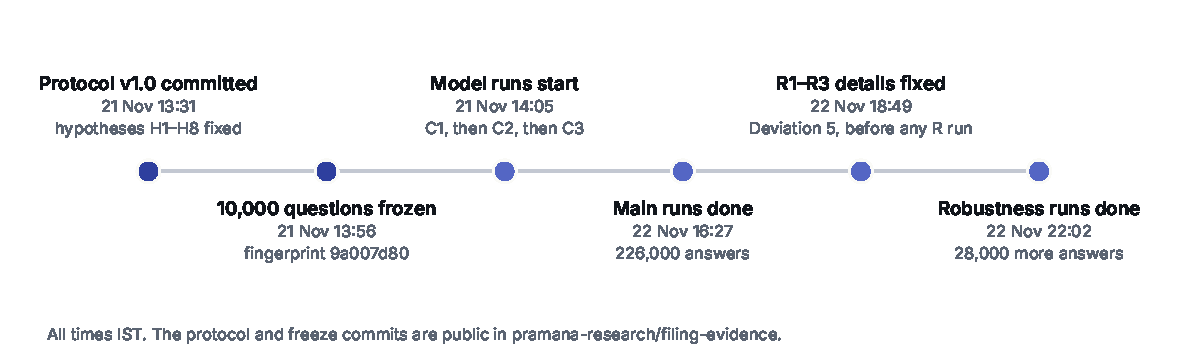
\includegraphics[width=\linewidth]{timeline.pdf}
\caption{The study in time. The protocol and the frozen questions were committed publicly before any model ran; the robustness checks were fully specified before any of them ran.}
\end{figure}
\paragraph{Companies and filings.} Ten sectors of ten companies each, chosen because their statements are laid out differently: banks, insurance, real estate, utilities, oil and gas, metals and mining, healthcare, technology, media and telecom. For each company we took its most recent 10-K and 10-Q from SEC EDGAR \citep{sec_edgar}: 200 filings. No company or datapoint from Filing-Evidence is reused.
\paragraph{Questions and answer key.} Gold answers come from the filers' inline XBRL tags. Each question shows three pages: the answer page, a neighbouring page and a distractor. There are 1,000 questions per sector; 9{,}002 have an answer on the pages shown, and the rest test whether the model answers ``not found''. Page rendering, wording rules, prompt and checker are those of Filing-Evidence, unchanged.
\paragraph{Difficulty tags.} Computed by code before any run: where the unit is stated (row label, the line itself, a table or column header, a page header, or nowhere on the pages shown); the number of figures on the evidence line; whether the answer is the first figure or a later one; the period length; and whether the amount uses a word scale (``\$12.6 billion'').
\paragraph{Outcomes.} \emph{Correct}: right value, and the quote passes every check. \emph{Confident-wrong}: wrong value, but the quote passes every check. \emph{Caught-wrong}: wrong value, and a check fails. \emph{Unverifiable-right}: right value, but the quote is unusable. \emph{Missed}: the model says ``not found'' although the number is there. For numbers that are absent, the outcome is \emph{abstained correctly} or \emph{invented}.

\section{Models and setups}
The ten models of Filing-Evidence at the same pinned revisions, plus Qwen3-8B as a supplementary model, served with vLLM~0.33 \citep{kwon2023vllm} on one RTX~4090 capped at 450\,W, temperature~0. Plain (C1) and check-and-retry (C2) run on all 10{,}000 questions. Thinking (C3) runs on a stratified 1{,}000-question subset for the six models with a reasoning mode, with up to 8{,}192 new tokens. Statistics: 95\% Wilson intervals \citep{wilson1927}; paired exact McNemar tests \citep{mcnemar1947}; Holm correction \citep{holm1979}; Kendall's $\tau$ \citep{kendall1938}. In total 254{,}000 answers.

\section{Does the sector matter? (RQ1, H1)}
\begin{figure}[H]
\centering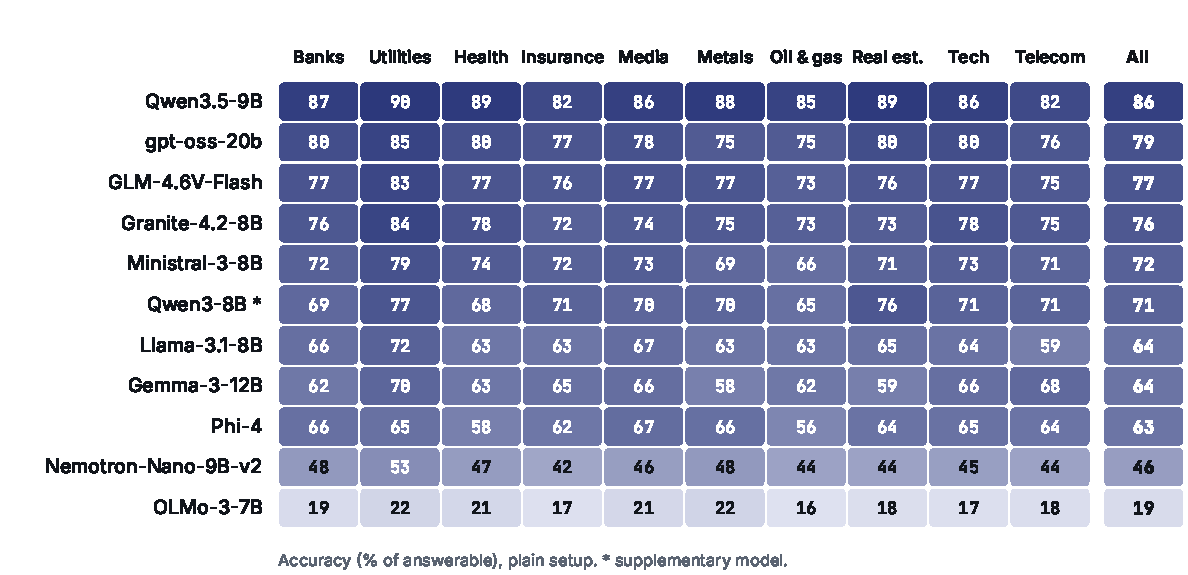
\includegraphics[width=.92\linewidth]{sector_heatmap.pdf}
\caption{Accuracy (\% of answerable questions) by model and sector, plain setup. Rows differ far more than columns. * supplementary model.}
\end{figure}
Pooled over the ten main models, accuracy ranges from 61.2\% (oil \& gas) to 70.2\% (utilities), a spread of 9 points, against 67 points between the best and worst model. The pre-registered test is a logistic regression of correctness on sector with a model fixed effect and standard errors clustered by company: $\chi^2(9) = 15.5$, $p = 0.08$. \textbf{H1 is not supported}: companies within a sector differ as much as sectors do.

\paragraph{The exception that wasn't (exploratory).} Confident-wrong rates vary more by sector than accuracy does. Oil and gas stands out at 15.5\% of answerable questions. The reason is specific: 14\% of its questions have no unit stated on the pages shown (the scale appears only elsewhere in the filing), against 0--8\% in other sectors. Those questions are answered confident-wrong 48\% of the time. Without them, oil and gas falls to 10.1\%, in line with other sectors (Figure~\ref{fig:unitless}).
\begin{figure}[H]
\centering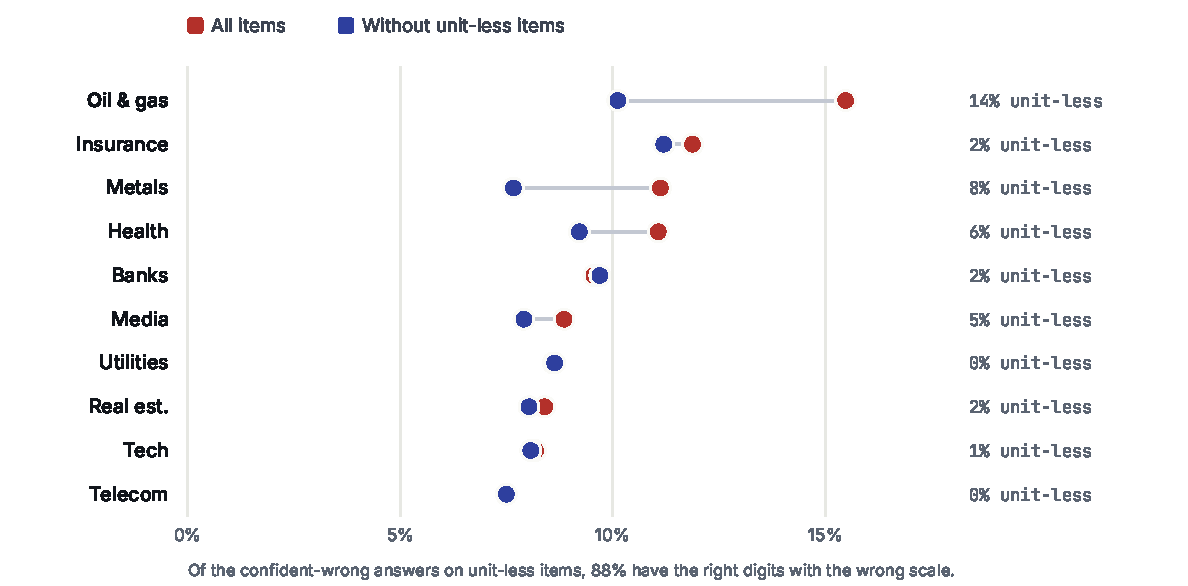
\includegraphics[width=.86\linewidth]{unitless.pdf}
\caption{Confident-wrong rate by sector, with all items and without items whose unit is stated nowhere on the pages shown.}\label{fig:unitless}
\end{figure}

\section{What makes a number hard? (RQ2, H2--H6)}
All five pre-registered hypotheses about the tags are supported. Each is a term in one logistic regression on all tags with a model fixed effect and standard errors clustered by company (89{,}780 answers, plain setup, ten main models), so each effect is estimated holding the others fixed (Table~\ref{tab:tags}, Figure~\ref{fig:forest}).
\begin{table}[H]\centering\small
\caption{Pre-registered tag hypotheses. Odds ratios with 95\% intervals; $p$ values Holm-corrected across H1--H8.}\label{tab:tags}
\begin{tabular}{p{.47\linewidth}rrr}\toprule
Hypothesis (outcome) & Odds ratio & 95\% CI & Holm $p$\\\midrule
H2 Unit away from the figure (confident-wrong) & 2.19 & 1.43--3.36 & <0.001\\
H3 Each extra figure on the line (correct) & 0.86 & 0.82--0.91 & <0.001\\
H4 Answer is a later figure (correct) & 0.69 & 0.64--0.74 & <0.001\\
H5 10-Q year-to-date vs three months (correct) & 0.72 & 0.62--0.82 & <0.001\\
H6 Word scale: unverifiable-right vs confident-wrong & 6.62 & 4.95--8.86 & <0.001\\
\bottomrule\end{tabular}
\end{table}
\begin{itemize}
\item \textbf{H2.} With the unit in a table or page header rather than the row label, confident-wrong rises from 4.4\% to 9.3\%; with no unit on the page it reaches 41\%.
\item \textbf{H3.} Accuracy falls from 71\% on two-figure lines to 42\% on lines with six or more.
\item \textbf{H4.} 70\% when the answer is the line's first figure, 60\% otherwise.
\item \textbf{H5.} In 10-Qs, 69\% for three-month figures, 61\% for six- and nine-month figures.
\item \textbf{H6.} Amounts written with a word scale fail mostly as unverifiable-right (1{,}840) rather than confident-wrong (354): models restate the value in other units, so the quote no longer matches.
\end{itemize}
\begin{figure}[H]
\centering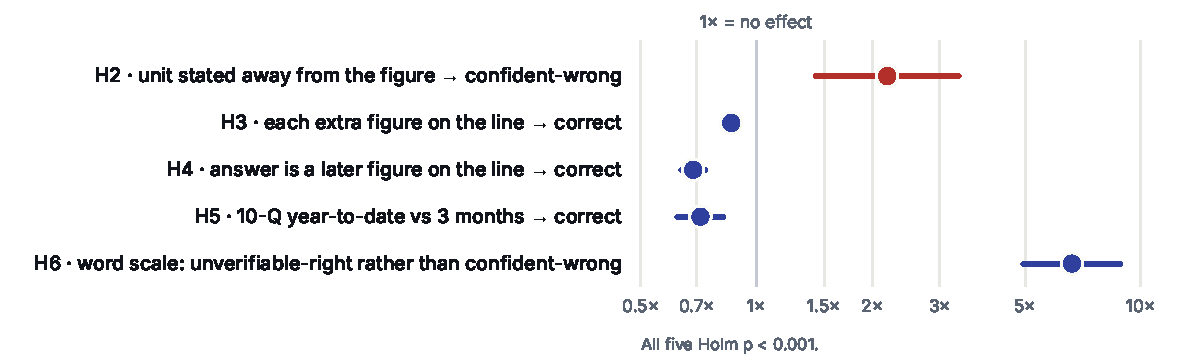
\includegraphics[width=.92\linewidth]{tag_forest.pdf}
\caption{Odds ratios with 95\% intervals for H2--H6.}\label{fig:forest}
\end{figure}
\paragraph{Mechanism: scale guessing.} Of the confident-wrong answers on numbers whose unit is stated nowhere on the page, 88\% have exactly the right digits with the wrong scale, for example ``52,611 in thousands'' where the filing means millions. The quote passes because the digits match; only knowing the unit can catch the error.

\section{Do the earlier findings hold? (RQ3, H7)}
\begin{figure}[H]
\centering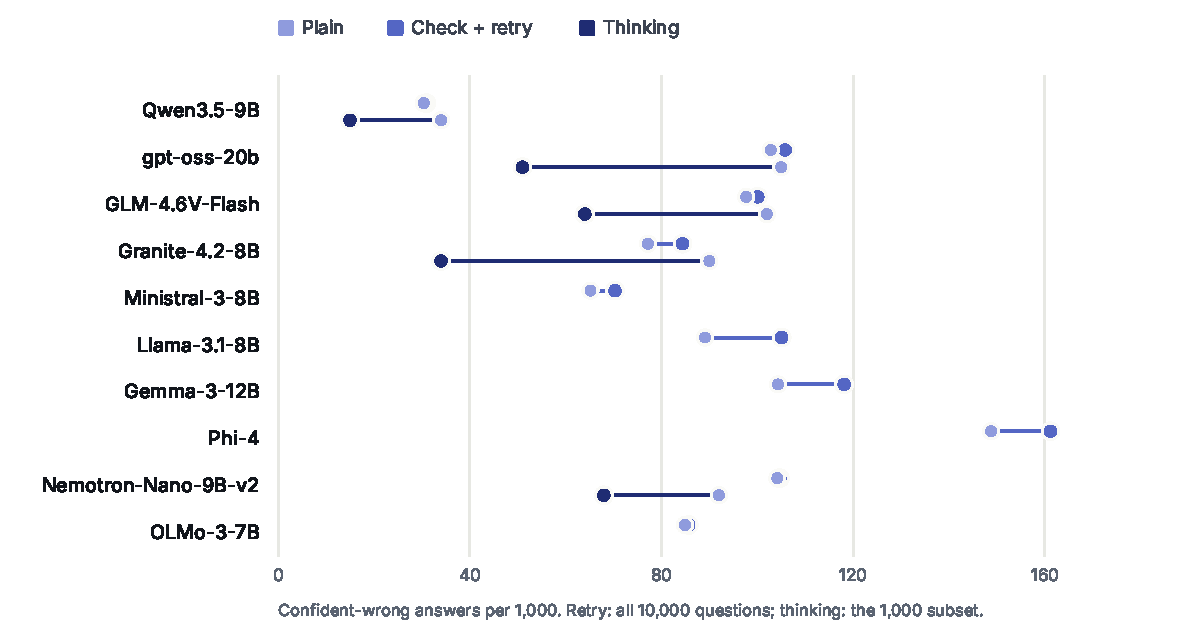
\includegraphics[width=.92\linewidth]{h7_arrows.pdf}
\caption{Confident-wrong answers per 1{,}000 in the plain setup and after check-and-retry (all questions) or thinking (the subset).}
\end{figure}
Yes. Thinking lowers confident-wrong answers significantly for 4 of the 5 main models with a reasoning mode (paired exact McNemar, Holm-corrected within model). Pooled, 299 answers stop being confident-wrong and 108 start. Check-and-retry never lowers them, and raises them significantly for 8 of 10 models while raising accuracy for 9: told that its quote failed, a model often finds another line containing its wrong number. \textbf{H7 is supported.} One exception: Qwen3.5-9B's accuracy fell with thinking (743 $\rightarrow$ 689 of 900), because 204 of its 1{,}000 answers hit the pre-registered 8{,}192-token limit; its confident-wrong answers still fell (34 $\rightarrow$ 15).

\section{Robustness}
Three checks, specified in full before any of them ran, all in the plain setup on the 1{,}000-question subset (Table~\ref{tab:robust}).
\paragraph{R3: repeat run.} The identical configuration run again changes the outcome of 0.6\%--3.4\% of questions for the three models tested, with no significant change in accuracy or confident-wrong.
\paragraph{R2: a different prompt.} New wording and a different worked example leave the model ranking almost unchanged (Kendall's $\tau = 0.87$). The two weakest models, Nemotron-Nano-9B-v2 and OLMo-3-7B, lose accuracy and gain confident-wrong answers under the new wording.
\paragraph{R1: Markdown tables (H8).} Tables rendered as Markdown, one row per line with column headers first. Wrong-period-or-column errors fall from 349 to 286 (pooled exact McNemar, $p = <0.001$): \textbf{H8 is supported}, and confident-wrong falls for every model. But strict accuracy collapses for most models, because many quote the row without its pipes and the pre-registered check, applied to the page text exactly as shown, rejects the quote; the ranking scrambles ($\tau = 0.20$). Grading R1 a second time with the pipes ignored, a decision made after seeing these results and therefore exploratory, removes most of the collapse and restores the ranking ($\tau = 0.87$). The best models read Markdown tables as well as flat text; the others lose up to 13 points. The tag effects of H2--H4 keep their direction under R1 and R2.
\begin{figure}[H]
\centering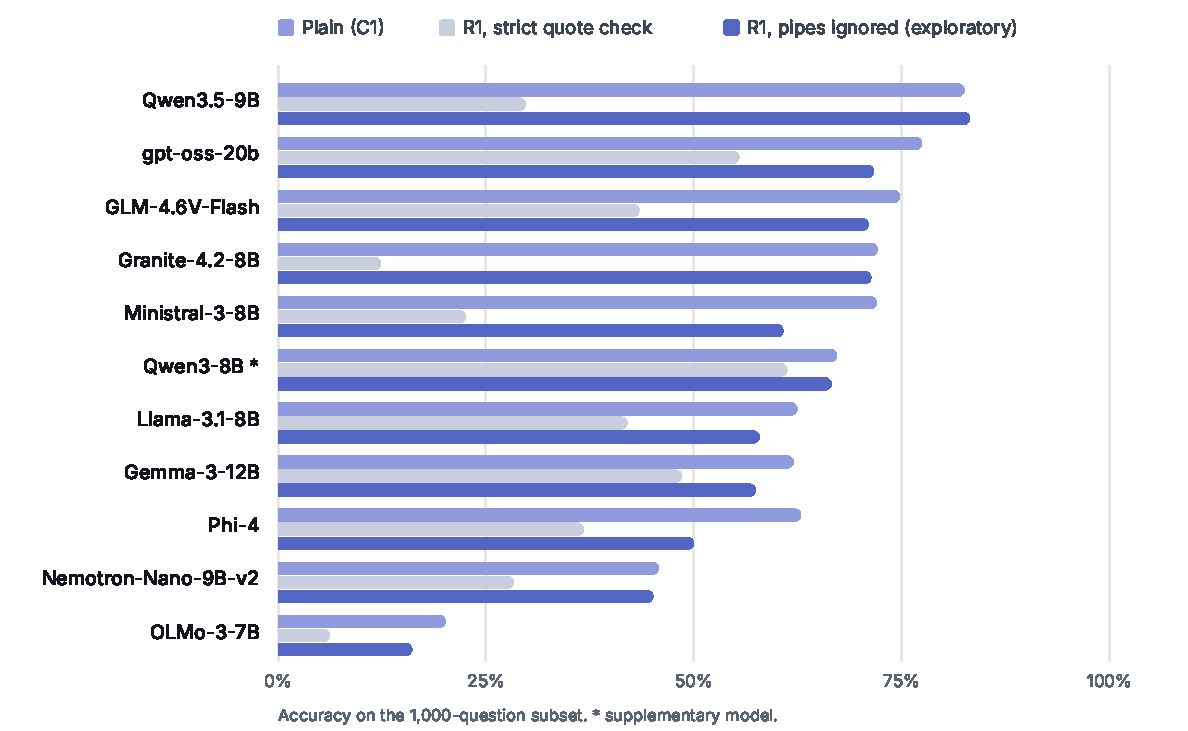
\includegraphics[width=.92\linewidth]{r1_bars.pdf}
\caption{Accuracy on the subset: plain setup, Markdown tables under the strict quote check, and Markdown tables with pipes ignored (exploratory).}
\end{figure}
\begin{table}[H]\centering\footnotesize
\caption{Robustness checks against the plain setup on the subset. Correct of 900 answerable; confident-wrong (CW) of 1{,}000. R1$^\ast$ ignores pipes in the quote check (exploratory). Supplementary model marked *.}\label{tab:robust}
\begin{tabular}{lrrrrrr}\toprule
Model & C1 & R1 & R1$^\ast$ & R2 & CW C1 & CW R1$^\ast$\\\midrule
Qwen3.5-9B & 743 & 268 & 749 & 715 & 34 & 32\\
gpt-oss-20b & 697 & 499 & 645 & 684 & 105 & 96\\
GLM-4.6V-Flash & 673 & 391 & 639 & 674 & 102 & 94\\
Granite-4.2-8B & 649 & 111 & 642 & 629 & 90 & 68\\
Ministral-3-8B & 648 & 203 & 547 & 633 & 52 & 47\\
Llama-3.1-8B & 562 & 378 & 521 & 524 & 92 & 73\\
Gemma-3-12B & 558 & 437 & 517 & 581 & 95 & 90\\
Phi-4 & 566 & 331 & 450 & 529 & 152 & 107\\
Nemotron-Nano-9B-v2 & 412 & 255 & 406 & 339 & 92 & 79\\
OLMo-3-7B & 181 & 56 & 145 & 89 & 75 & 51\\
Qwen3-8B * & 605 & 551 & 599 & 612 & 103 & 97\\
\bottomrule\end{tabular}
\end{table}

\section{Cost and trust on one GPU (exploratory)}
GPU energy per 1{,}000 answers, taken from the card's energy counter over each model's R2 run (plain-setup settings), ranges from 24\,Wh (gpt-oss-20b) to 51\,Wh (Nemotron-Nano-9B-v2): about US\$0.004--0.009 at \$0.17 per kWh. Repeat runs agree within 6\%. These are GPU board figures only. We also ran 4-bit builds of three models on the subset: Qwen3.5-9B loses accuracy (743 $\rightarrow$ 711, significant) without a significant rise in confident-wrong (34 $\rightarrow$ 42); for the other two, neither changes significantly.
\begin{figure}[H]
\centering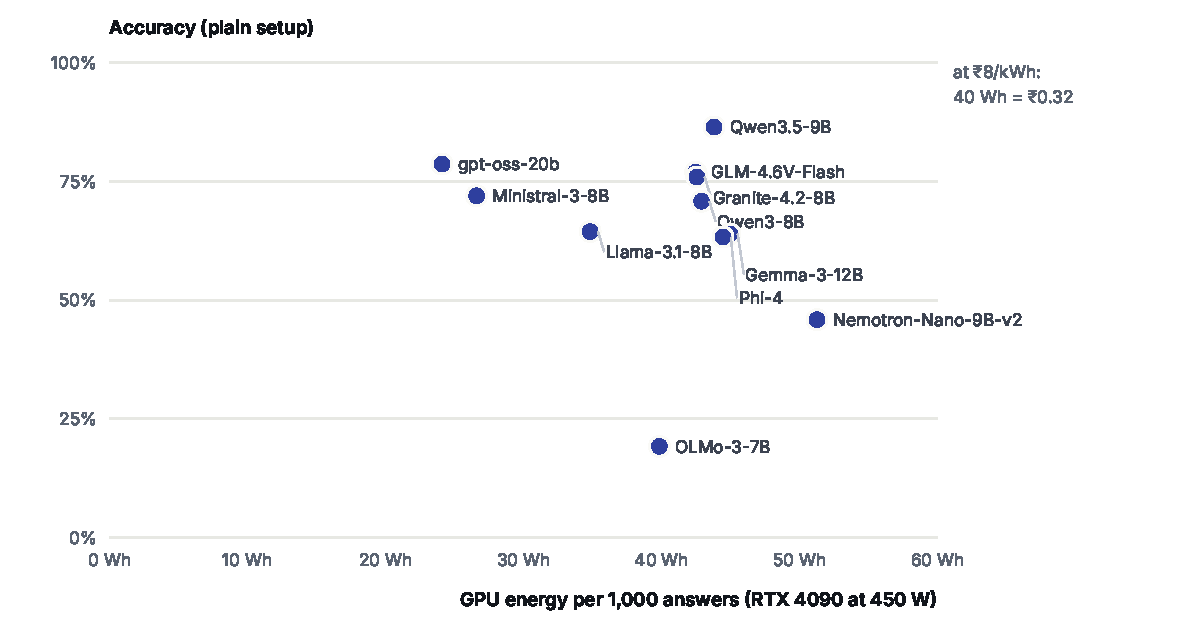
\includegraphics[width=.86\linewidth]{cost_scatter.pdf}
\caption{Plain-setup accuracy against GPU energy per 1{,}000 answers.}
\end{figure}

\section{Discussion}
\paragraph{Look at the line, not the industry.} Errors concentrate in numbers whose unit sits in a header, on crowded lines, in later columns and in year-to-date periods, in every sector.
\paragraph{Give the model the unit.} The most dangerous case is a number whose unit is not on the page at all: the model guesses, and a digit-based check passes the guess. A reader system should carry the document's scale statement with every page, or verify the scale separately.
\paragraph{Think, don't retry.} Thinking reduces confident-wrong answers; retrying after a failed check increases them. The thinking budget must be large enough not to cut answers off.
\paragraph{Make the evidence check layout-tolerant.} A strict character-for-character check punishes formatting, not reading. Comparing the words and figures of a quote keeps the guarantee and removes the artefact.

\section{Limitations}
The tag effects are observational: we did not move a unit from a row label to a header and re-ask, although the regression holds the other tags fixed and R1 is a true intervention on layout. One hardware and serving configuration (RTX~4090 at 450\,W, vLLM~0.33, temperature~0). A fixed thinking budget cut off a fifth of Qwen3.5-9B's thinking answers. R1's rendering is imperfect: in 75\% of tables with a header, the last header row has as many cells as the first data row. The oil-and-gas analysis, the pipe-insensitive R1 grading and the cost-and-trust extension are exploratory. US filings only.

\section{Reproducibility and deviations}
The protocol, its seven logged deviations, the code, the frozen questions (fingerprint \texttt{9a007d80}), the Markdown pages of R1 (\texttt{7cdf066e}) and every model reply are public: code at \url{https://github.com/pramana-research/filing-evidence-sectors}, data at \url{https://huggingface.co/datasets/pramana-research/filing-evidence-sectors}. In a fresh clone, re-grading every stored reply reproduces every run summary byte for byte. The pre-registration commits are public in the Filing-Evidence repository. Deviations: (1)~a sampling rule changed to reach 10{,}000 questions, before any run; (2)~the cost-and-trust extension, exploratory; (3)~analysis code written after the runs, implementing the registered plan; (4)~the study moved to its own repository; (5)~details of R1--R3 and the 4-bit runs fixed before those runs; (6)~the pipe-insensitive R1 grading, exploratory; (7)~energy from the GPU counter rather than dedicated runs.

\section{Conclusion}
Across ten sectors and 254{,}000 answers, the industry a number comes from matters little; how it is printed matters a great deal. Units away from the figure, crowded lines, later columns and year-to-date periods predict errors, and a number with no unit on the page invites a confident wrong guess that a quote check cannot see. Thinking helps, retrying does not, and evidence checks must tolerate layout.

\section*{Acknowledgements and disclaimer}
This is an independent community research report written in a personal capacity; it does not represent the views of any employer. It is not affiliated with or endorsed by any company or model developer named here. Results describe specific model versions under one fixed setup. Nothing here is financial, investment or legal advice.

\begin{thebibliography}{15}
\bibitem[Bohnet et~al.(2022)]{bohnet2022attributed} B. Bohnet et al. Attributed question answering: Evaluation and modeling for attributed large language models. \emph{arXiv:2212.08037}, 2022.
\bibitem[Chen et~al.(2021)]{chen2021finqa} Z. Chen et al. FinQA: A dataset of numerical reasoning over financial data. In \emph{Proceedings of EMNLP}, 2021.
\bibitem[Gao et~al.(2023)]{gao2023alce} T. Gao, H. Yen, J. Yu, and D. Chen. Enabling large language models to generate text with citations. In \emph{Proceedings of EMNLP}, 2023.
\bibitem[Holm(1979)]{holm1979} S. Holm. A simple sequentially rejective multiple test procedure. \emph{Scandinavian Journal of Statistics}, 6(2):65--70, 1979.
\bibitem[Islam et~al.(2023)]{islam2023financebench} P. Islam et al. FinanceBench: A new benchmark for financial question answering. \emph{arXiv:2311.11944}, 2023.
\bibitem[Kendall(1938)]{kendall1938} M. G. Kendall. A new measure of rank correlation. \emph{Biometrika}, 30(1--2):81--93, 1938.
\bibitem[Kwon et~al.(2023)]{kwon2023vllm} W. Kwon et al. Efficient memory management for large language model serving with PagedAttention. In \emph{Proceedings of SOSP}, 2023.
\bibitem[Liu et~al.(2023)]{liu2023verifiability} N. F. Liu, T. Zhang, and P. Liang. Evaluating verifiability in generative search engines. In \emph{Findings of EMNLP}, 2023.
\bibitem[McNemar(1947)]{mcnemar1947} Q. McNemar. Note on the sampling error of the difference between correlated proportions or percentages. \emph{Psychometrika}, 12(2):153--157, 1947.
\bibitem[Nandula(2026)]{nandula2026filingevidence} K. Nandula. Show your work: Can small open models read SEC filings with evidence a machine can check? \emph{arXiv:2611.24990}, 2026.
\bibitem[Reddy et~al.(2024)]{reddy2024docfinqa} V. Reddy et al. DocFinQA: A long-context financial reasoning dataset. In \emph{Proceedings of ACL}, 2024.
\bibitem[{SEC}(2026)]{sec_edgar} U.S. Securities and Exchange Commission. EDGAR. \url{https://www.sec.gov/edgar}, 2026.
\bibitem[Wilson(1927)]{wilson1927} E. B. Wilson. Probable inference, the law of succession, and statistical inference. \emph{Journal of the American Statistical Association}, 22(158):209--212, 1927.
\bibitem[{XBRL International}(2013)]{xbrl2013inline} XBRL International. Inline XBRL Part 1: Specification 1.1, 2013.
\bibitem[Zhu et~al.(2021)]{zhu2021tatqa} F. Zhu et al. TAT-QA: A question answering benchmark on a hybrid of tabular and textual content in finance. In \emph{Proceedings of ACL-IJCNLP}, 2021.
\end{thebibliography}

\clearpage
\appendix
\section{Accuracy and confident-wrong by model}\label{app:models}
\begin{table}[H]\centering\footnotesize
\caption{Plain (C1) and check-and-retry (C2) on all 10{,}000 questions; thinking (C3) on the subset. Accuracy is the share of answerable questions; confident-wrong (CW) the share of all questions. Supplementary model marked *.}
\begin{tabular}{lrrrrr}\toprule
Model & Acc C1 & CW C1 & Acc C2 & CW C2 & CW C1$\to$C3 (subset)\\\midrule
Qwen3.5-9B & 86.4\% & 3.0\% & 87.0\% & 3.1\% & 34 $\rightarrow$ 15\\
gpt-oss-20b & 78.6\% & 10.3\% & 80.6\% & 10.6\% & 105 $\rightarrow$ 51\\
GLM-4.6V-Flash & 76.9\% & 9.8\% & 78.3\% & 10.0\% & 102 $\rightarrow$ 64\\
Granite-4.2-8B & 75.9\% & 7.7\% & 78.4\% & 8.4\% & 90 $\rightarrow$ 34\\
Ministral-3-8B & 71.9\% & 6.5\% & 74.5\% & 7.0\% & --\\
Llama-3.1-8B & 64.4\% & 8.9\% & 68.7\% & 10.5\% & --\\
Gemma-3-12B & 63.9\% & 10.4\% & 66.7\% & 11.8\% & --\\
Phi-4 & 63.3\% & 14.9\% & 65.5\% & 16.1\% & --\\
Nemotron-Nano-9B-v2 & 45.9\% & 10.4\% & 46.0\% & 10.5\% & 92 $\rightarrow$ 68\\
OLMo-3-7B & 19.2\% & 8.5\% & 19.2\% & 8.6\% & --\\
Qwen3-8B * & 70.8\% & 9.4\% & 72.7\% & 10.0\% & 103 $\rightarrow$ 58\\
\bottomrule\end{tabular}
\end{table}

\section{Additional figures}
\begin{figure}[H]
\centering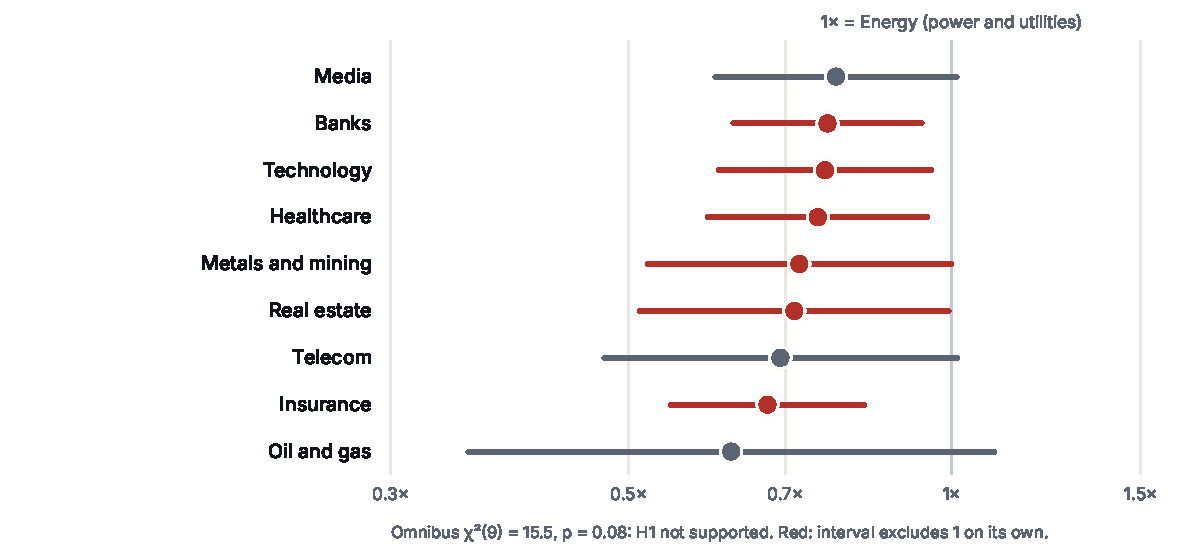
\includegraphics[width=.86\linewidth]{sector_or.pdf}
\caption{Odds of a correct answer by sector relative to the easiest sector (H1).}
\end{figure}
\begin{figure}[H]
\centering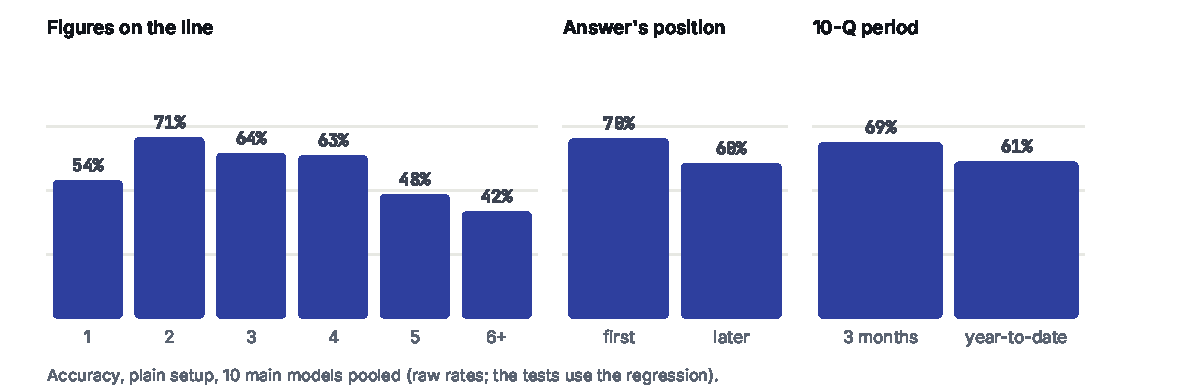
\includegraphics[width=.92\linewidth]{tag_rates.pdf}
\caption{Raw accuracy by figures on the line, position of the answer, and 10-Q period.}
\end{figure}
\begin{figure}[H]
\centering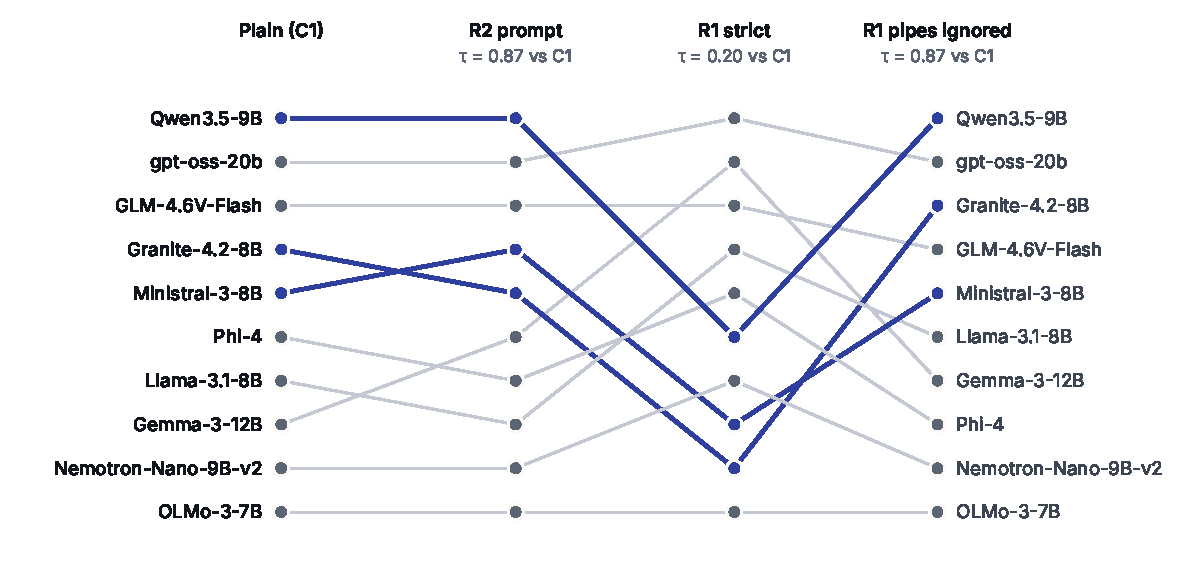
\includegraphics[width=.86\linewidth]{rank_slope.pdf}
\caption{Model ranks by accuracy under each robustness check.}
\end{figure}
\begin{figure}[H]
\centering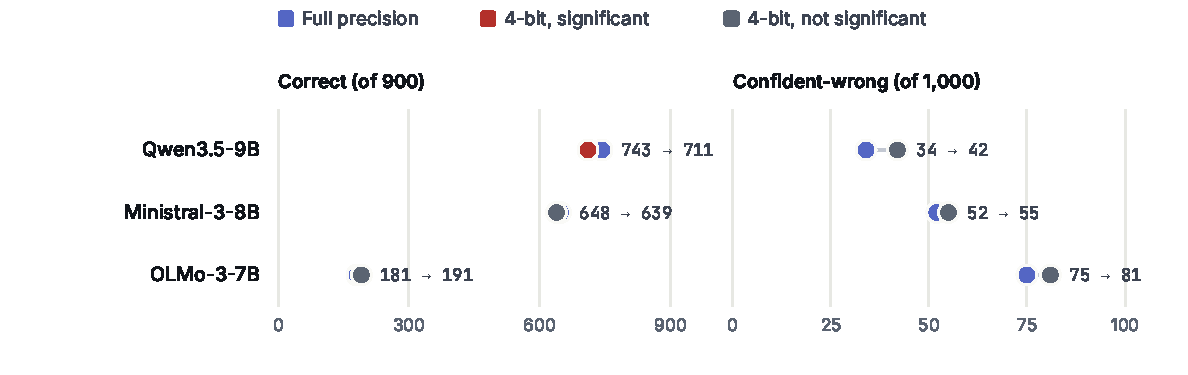
\includegraphics[width=.86\linewidth]{quant_pairs.pdf}
\caption{Full precision against the 4-bit build of the same model, plain setup, subset.}
\end{figure}

\end{document}